\documentclass[12pt,a4paper]{article}

% ─── Page Layout ───────────────────────────────────────────────────────────────
\usepackage[a4paper, margin=0.8in, headheight=14pt]{geometry}

% ─── Fonts (XeLaTeX) ───────────────────────────────────────────────────────────
\usepackage{fontspec}
\usepackage{unicode-math}
\setmainfont{TeX Gyre Pagella}
\setmonofont[Scale=0.88]{TeX Gyre Cursor}
\setmathfont{Latin Modern Math}

% ─── Packages ──────────────────────────────────────────────────────────────────
\usepackage{xcolor}
\usepackage{colortbl}
\usepackage{titlesec}
\usepackage{enumitem}
\usepackage{tabularx}
\usepackage{booktabs}
\usepackage{array}
\usepackage{amsmath}
\usepackage{tikz}
\usetikzlibrary{shapes.geometric, arrows.meta, positioning, calc, fit, decorations.pathreplacing}
\usepackage{tcolorbox}
\tcbuselibrary{skins, breakable}
\usepackage{hyperref}
\usepackage{fancyhdr}
\usepackage{graphicx}
\usepackage{microtype}
\hyphenpenalty=10000
\exhyphenpenalty=10000
\sloppy
\usepackage{caption}
\usepackage{setspace}
\usepackage{multirow}
\usepackage{tocloft}

% ─── Q&A helper ────────────────────────────────────────────────────────────────
\newcommand{\Q}[1]{\textbf{#1}\par\noindent\ignorespaces}

% ─── Colour Palette ────────────────────────────────────────────────────────────
\definecolor{myred}{RGB}{196,30,58}
\definecolor{mydark}{RGB}{30,30,50}
\definecolor{mygreen}{RGB}{14,120,80}
\definecolor{myteal}{RGB}{0,130,140}
\definecolor{myamber}{RGB}{180,100,0}
\definecolor{mypurple}{RGB}{100,30,160}
\definecolor{mygray}{RGB}{246,247,249}
\definecolor{mgframe}{RGB}{180,185,200}
\definecolor{watermark}{RGB}{145,150,170}
\definecolor{hdrred}{RGB}{250,232,235}
\definecolor{hdrgreen}{RGB}{220,244,233}
\definecolor{hdrteal}{RGB}{220,242,244}
\definecolor{hdramber}{RGB}{253,242,215}
\definecolor{hdrpurple}{RGB}{238,228,255}

% ─── Section Formatting ────────────────────────────────────────────────────────
\titleformat{\section}
  {\large\bfseries\color{myred}}{\thesection.}{0.5em}{}
  [\vspace{1pt}{\color{myred}\rule{\linewidth}{0.8pt}}]
\titleformat{\subsection}
  {\normalsize\bfseries\color{myteal}}{\thesubsection}{0.5em}{}
\titlespacing*{\section}{0pt}{18pt}{7pt}
\titlespacing*{\subsection}{0pt}{11pt}{4pt}

% ─── Paragraph ─────────────────────────────────────────────────────────────────
\setlength{\parindent}{0pt}
\setlength{\parskip}{4pt}

% ─── TOC Styling ───────────────────────────────────────────────────────────────
\renewcommand{\cfttoctitlefont}{\large\bfseries\color{myred}}
\renewcommand{\cftaftertoctitle}{\par\noindent{\color{myred}\rule{\linewidth}{0.8pt}}}
\setlength{\cftbeforetoctitleskip}{0pt}
\setlength{\cftaftertoctitleskip}{6pt}
\renewcommand{\cftsecfont}{\normalsize\bfseries\color{mydark}}
\renewcommand{\cftsecpagefont}{\normalsize\bfseries\color{mydark}}
\renewcommand{\cftsecleader}{\cftdotfill{\cftdotsep}}
\setlength{\cftbeforesecskip}{7pt}
\renewcommand{\cftsubsecfont}{\small\color{mydark}}
\renewcommand{\cftsubsecpagefont}{\small\color{mydark}}
\setlength{\cftbeforesubsecskip}{3pt}
\setlength{\cftsubsecindent}{1.4em}

% ─── Table helpers ─────────────────────────────────────────────────────────────
\renewcommand{\arraystretch}{1.45}
\setlength{\tabcolsep}{6pt}
\arrayrulecolor{mydark}
\newcolumntype{B}[1]{>{\small\bfseries\raggedright\arraybackslash}m{#1}}
\newcolumntype{Y}{>{\small\raggedright\arraybackslash}X}
\renewcommand{\tabularxcolumn}[1]{m{#1}}

% ─── Header / Footer ───────────────────────────────────────────────────────────
\pagestyle{fancy}
\fancyhf{}
\fancyhead[L]{\small\color{myred}\textbf{PE-EC801C}\;\color{mydark}--- Error Correcting Codes}
\fancyhead[R]{\small\color{myteal}\textbf{Module 5 Notes}}
\fancyfoot[C]{\small\color{mydark}\thepage}
\fancyfoot[R]{\small\color{watermark}\textit{\copyright\ Biraj}}
\renewcommand{\headrulewidth}{0.5pt}
\renewcommand{\footrulewidth}{0.3pt}

% ─── Hyperref ──────────────────────────────────────────────────────────────────
\hypersetup{
  colorlinks=true, linkcolor=myteal, urlcolor=myteal,
  pdfauthor={Biraj Sarkar},
  pdftitle={PE-EC801C --- Module 5 Notes}
}

% ─── tcolorbox styles ──────────────────────────────────────────────────────────
\tcbset{
  tikzbox/.style={
    colback=mygray, colframe=mgframe, boxrule=0.6pt, arc=4pt,
    left=8pt, right=8pt, top=6pt, bottom=6pt,
    colbacktitle=mgframe, coltitle=mydark,
    fonttitle=\small\bfseries
  },
  defbox/.style={
    colback=hdrgreen, colframe=mygreen, boxrule=0.8pt, arc=4pt,
    left=9pt, right=9pt, top=6pt, bottom=6pt,
    colbacktitle=mygreen, coltitle=white,
    fonttitle=\small\bfseries
  },
  formulabox/.style={
    colback=hdrteal, colframe=myteal, boxrule=0.8pt, arc=4pt,
    left=9pt, right=9pt, top=7pt, bottom=7pt,
    colbacktitle=myteal, coltitle=white,
    fonttitle=\small\bfseries
  },
  examplebox/.style={
    colback=hdramber, colframe=myamber, boxrule=0.8pt, arc=4pt,
    left=9pt, right=9pt, top=6pt, bottom=6pt,
    colbacktitle=myamber, coltitle=white,
    fonttitle=\small\bfseries
  },
  masonbox/.style={
    colback=hdrpurple, colframe=mypurple, boxrule=0.8pt, arc=4pt,
    left=9pt, right=9pt, top=6pt, bottom=6pt,
    colbacktitle=mypurple, coltitle=white,
    fonttitle=\small\bfseries
  },
  exambox/.style={
    colback=hdrpurple, colframe=mypurple, boxrule=1pt, arc=5pt,
    left=10pt, right=10pt, top=8pt, bottom=8pt,
    colbacktitle=mypurple, coltitle=white,
    fonttitle=\bfseries,
    breakable, title after break={\textbf{Frequently Asked / Viva Questions (contd.)}}}
}
\tcbset{breakable}
\tcbset{after={\color{black}}}

% ─── TikZ styles ───────────────────────────────────────────────────────────────
\tikzset{
  stepnode/.style={rectangle, draw=myteal, fill=hdrteal,
    text width=3.4cm, align=center, minimum height=1.0cm,
    font=\small\bfseries, rounded corners=4pt, line width=0.8pt},
  flowarrow/.style={-Stealth, thick, color=mydark},
  arrow/.style={-Stealth, thick, color=mydark},
  reg/.style={rectangle, draw=myteal, fill=hdrteal,
    minimum width=0.8cm, minimum height=0.8cm, align=center,
    font=\small\bfseries, line width=0.7pt},
  adder/.style={circle, draw=myamber, fill=hdramber,
    minimum size=0.45cm, font=\small\bfseries, line width=0.8pt, inner sep=0pt},
  mult/.style={circle, draw=mypurple, fill=hdrpurple,
    minimum size=0.45cm, font=\small, line width=0.7pt, inner sep=0pt},
  line/.style={thick, color=mydark},
  state/.style={circle, draw=myteal, fill=hdrteal,
    minimum size=0.9cm, font=\small\bfseries, line width=0.8pt},
  trellisnode/.style={circle, fill=mydark, inner sep=1.5pt}
}

% ═══════════════════════════════════════════════════════════════════════════════
\begin{document}
% ═══════════════════════════════════════════════════════════════════════════════

\begin{center}
  {\LARGE\bfseries\color{myred} PE-EC801C --- Error Correcting Codes}\\[5pt]
  {\normalsize\color{mydark} Semester VIII \quad$\bullet$\quad 3L:0T:0P \quad$\bullet$\quad 3 Credits}\\[3pt]
  {\normalsize\color{myteal}\textbf{Module 5: Convolutional Codes and Decoding}}\\[3pt]
  {\small\color{mydark} CGEC \;$|$\; B.Tech ECE (2023--27) \;$|$\; \textit{Biraj Sarkar}}
\end{center}
\vspace{2pt}
\noindent{\color{myred}\rule{\linewidth}{1.5pt}}
\vspace{2pt}

\hypersetup{linkcolor=mydark}
\tableofcontents
\hypersetup{linkcolor=myteal}
\newpage

% ===============================================================================
\section{Introduction to Convolutional Codes}
% ===============================================================================

Unlike linear block codes, which segment the incoming message sequence into independent blocks of length $k$, \textbf{convolutional codes} process the message continuously. The coded output depends not only on the current input block but also on a finite number of previous input blocks stored in memory.

\subsection{Core Parameters}
A convolutional encoder is characterized by three main parameters:
\begin{enumerate}[leftmargin=*, itemsep=3pt]
  \item \textbf{Code Rate (\texorpdfstring{$R$}{R}):} Defined as $R = k/n$, where $k$ input bits produce $n$ output bits in each encoding cycle.
  \item \textbf{Memory Stages (\texorpdfstring{$M$}{M}):} The number of delay elements (flip-flops) in the shift registers.
  \item \textbf{Constraint Length (\texorpdfstring{$K$}{K}):} There are two standard definitions:
    \begin{itemize}[leftmargin=*, itemsep=2pt]
      \item \textbf{System-Theoretic definition:} $K = M + 1$. This represents the maximum number of input cycles over which a single input bit can influence the encoder's output.
      \item \textbf{Alternative definition:} $K = L \cdot k$, where $L$ is the number of stages in the shift register.
    \end{itemize}
\end{enumerate}

\subsection{Mathematical Representations}
The encoding operation can be described in three algebraic formats:
\begin{tcolorbox}[defbox, title={\textbf{Mathematical Formulations of Convolutional Coding}}]
\begin{enumerate}[leftmargin=*, itemsep=3pt, topsep=0pt]
  \item \textbf{Impulse Response:} Let $h^{(j)} = (h^{(j)}_0, h^{(j)}_1, \dots)$ be the impulse response of the path from the input to output $j$. For input sequence $u = (u_0, u_1, \dots)$, the output $v^{(j)}$ is the discrete convolution:
    \[ v^{(j)}_t = \sum_{i=0}^M u_{t-i} h^{(j)}_i \]
  \item \textbf{Generator Matrix (\texorpdfstring{$G$}{G}):} A semi-infinite, Block-Toeplitz matrix of the form:
    \[ G = \begin{bmatrix} 
      G_0 & G_1 & G_2 & \dots & G_M & 0 & \dots \\
      0   & G_0 & G_1 & \dots & G_{M-1} & G_M & \dots \\
      0   & 0   & G_0 & \dots & G_{M-2} & G_{M-1} & \dots \\
      \vdots & \vdots & \vdots & \ddots & \vdots & \vdots & \ddots
    \end{bmatrix} \]
    where each $G_i$ is a $k \times n$ sub-matrix representing tap connections.
  \item \textbf{Generator Polynomials:} Tap connections for the $j$-th output are expressed as a polynomial in the delay operator $D$:
    \[ g^{(j)}(D) = g^{(j)}_0 \oplus g^{(j)}_1 D \oplus g^{(j)}_2 D^2 \oplus \dots \oplus g^{(j)}_M D^M \]
\end{enumerate}
\end{tcolorbox}

% ===============================================================================
\section{Structural Representations}
% ===============================================================================

Convolutional encoders are implemented using feed-forward shift registers and modulo-2 adders. They can be analyzed using three graphical models.

\begin{tcolorbox}[tikzbox, title={Feed-Forward Encoder for a Rate 1/2 (\texorpdfstring{$K=3$}{K=3}) Convolutional Code}]
\centering
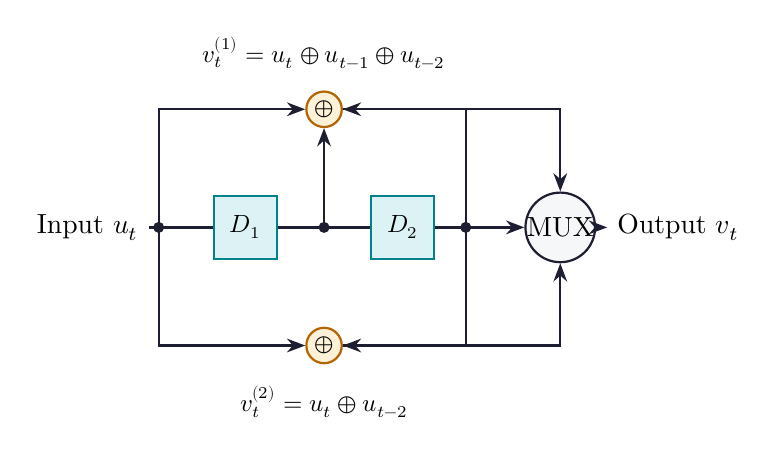
\begin{tikzpicture}[node distance=1.5cm, >=Stealth, thick]
  % Nodes
  \node (in) at (0,0) {Input $u_t$};
  \node[reg] (d1) at (2.0, 0) {$D_1$};
  \node[reg] (d2) at (4.0, 0) {$D_2$};
  
  % Modulo-2 adders
  \node[adder] (add1) at (3.0, 1.5) {$\oplus$};
  \node[adder] (add2) at (3.0, -1.5) {$\oplus$};

  % Output nodes
  \node[circle, draw=mydark, fill=mygray, minimum size=0.7cm, inner sep=0pt] (mux) at (6.0, 0) {MUX};
  \node (out) at (7.5, 0) {Output $v_t$};

  % Connections along main line
  \draw[line] (in) -- (d1);
  \draw[line] (d1) -- (d2);
  \draw[arrow] (d2) -- (mux);

  % Taps (coordinates along the line)
  \coordinate (tap0) at (0.9, 0);
  \coordinate (tap1) at (3.0, 0);
  \coordinate (tap2) at (4.8, 0);

  % Draw connection dots
  \fill[mydark] (tap0) circle (2pt);
  \fill[mydark] (tap1) circle (2pt);
  \fill[mydark] (tap2) circle (2pt);

  % Tap lines to Adder 1
  \draw[arrow] (tap0) |- (add1);
  \draw[arrow] (tap1) -- (add1);
  \draw[arrow] (tap2) |- (add1);

  % Tap lines to Adder 2
  \draw[arrow] (tap0) |- (add2);
  \draw[arrow] (tap2) |- (add2);

  % Adder to MUX
  \draw[arrow] (add1) -| (mux);
  \draw[arrow] (add2) -| (mux);
  \draw[arrow] (mux) -- (out);

  % Labels for outputs
  \node[above=0.15cm of add1] {\small $v^{(1)}_t = u_t \oplus u_{t-1} \oplus u_{t-2}$};
  \node[below=0.15cm of add2] {\small $v^{(2)}_t = u_t \oplus u_{t-2}$};
\end{tikzpicture}
\end{tcolorbox}

\subsection{State Transition Diagram}
A state transition diagram represents the encoder as a finite-state machine. The state is determined by the previous bits stored in the shift register: $S_t = (u_{t-1}, u_{t-2}, \dots, u_{t-M})$. For $M=2$, there are four possible states: $00$, $10$, $01$, and $11$.

\begin{tcolorbox}[tikzbox, title={State Transition Diagram (4-State, K=3 Encoder)}]
\centering
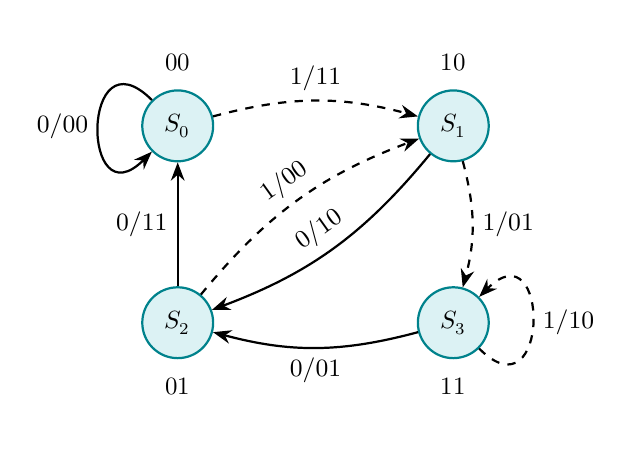
\begin{tikzpicture}[node distance=2.2cm, >=Stealth, thick]
  % Define states
  \node[state] (s0) at (0, 2) {$S_0$};
  \node[state] (s1) at (3.5, 2) {$S_1$};
  \node[state] (s2) at (0, -0.5) {$S_2$};
  \node[state] (s3) at (3.5, -0.5) {$S_3$};

  % Labels for states
  \node[above=0.1cm of s0] {\small $00$};
  \node[above=0.1cm of s1] {\small $10$};
  \node[below=0.1cm of s2] {\small $01$};
  \node[below=0.1cm of s3] {\small $11$};

  % Transitions
  % S0 loop
  \draw[->] (s0) to[out=135, in=225, looseness=5] node[left]{\small 0/00} (s0);
  % S0 to S1
  \draw[->, dashed] (s0) to[bend left=15] node[above]{\small 1/11} (s1);
  % S1 to S2
  \draw[->] (s1) to[bend left=15] node[above, sloped]{\small 0/10} (s2);
  % S1 to S3
  \draw[->, dashed] (s1) to[bend left=15] node[right]{\small 1/01} (s3);
  % S2 to S0
  \draw[->] (s2) to node[left]{\small 0/11} (s0);
  % S2 to S1
  \draw[->, dashed] (s2) to[bend left=15] node[above, sloped]{\small 1/00} (s1);
  % S3 to S2
  \draw[->] (s3) to[bend left=15] node[below]{\small 0/01} (s2);
  % S3 loop
  \draw[->, dashed] (s3) to[out=315, in=45, looseness=5] node[right]{\small 1/10} (s3);
\end{tikzpicture}
\par\vspace{3pt}\noindent
\small\textbf{Legend:} Solid lines represent transitions caused by input `0'. Dashed lines represent transitions caused by input `1'. Labels indicate \texttt{Input/Output}.
\end{tcolorbox}

\subsection{Tree Diagram}
The tree diagram represents all possible output paths starting from the initial state $00$. For each incoming bit, the path splits into two branches: the upper branch represents input $0$, and the lower branch represents input $1$. The diagram grows exponentially, making it suitable only for illustrating short sequences.

\begin{tcolorbox}[tikzbox, title={3-Level Tree Diagram Representation}]
\centering
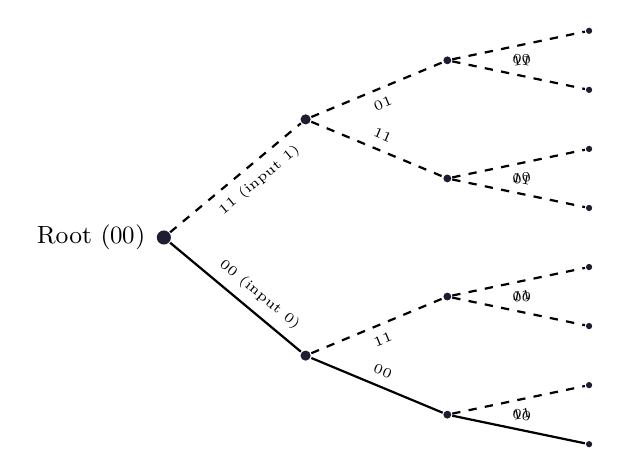
\begin{tikzpicture}[level distance=1.8cm,
  level 1/.style={sibling distance=3.0cm},
  level 2/.style={sibling distance=1.5cm},
  level 3/.style={sibling distance=0.75cm},
  grow=right, >=Stealth, thick]
  
  \node[circle, fill=mydark, inner sep=1.8pt, label=left:{\small Root ($00$)}] (root) {}
    child {
      node[circle, fill=mydark, inner sep=1.3pt] {}
      child {
        node[circle, fill=mydark, inner sep=1.0pt] {}
        child {
          node[circle, fill=mydark, inner sep=0.8pt] {}
          edge from parent node[above, sloped, pos=0.5] {\tiny 00}
        }
        child[dashed] {
          node[circle, fill=mydark, inner sep=0.8pt] {}
          edge from parent node[below, sloped, pos=0.5] {\tiny 11}
        }
        edge from parent node[above, sloped, pos=0.5] {\tiny 00}
      }
      child[dashed] {
        node[circle, fill=mydark, inner sep=1.0pt] {}
        child {
          node[circle, fill=mydark, inner sep=0.8pt] {}
          edge from parent node[above, sloped, pos=0.5] {\tiny 10}
        }
        child[dashed] {
          node[circle, fill=mydark, inner sep=0.8pt] {}
          edge from parent node[below, sloped, pos=0.5] {\tiny 01}
        }
        edge from parent node[below, sloped, pos=0.5] {\tiny 11}
      }
      edge from parent node[above, sloped, pos=0.6] {\tiny 00 (input 0)}
    }
    child[dashed] {
      node[circle, fill=mydark, inner sep=1.3pt] {}
      child {
        node[circle, fill=mydark, inner sep=1.0pt] {}
        child {
          node[circle, fill=mydark, inner sep=0.8pt] {}
          edge from parent node[above, sloped, pos=0.5] {\tiny 11}
        }
        child[dashed] {
          node[circle, fill=mydark, inner sep=0.8pt] {}
          edge from parent node[below, sloped, pos=0.5] {\tiny 00}
        }
        edge from parent node[above, sloped, pos=0.5] {\tiny 11}
      }
      child[dashed] {
        node[circle, fill=mydark, inner sep=1.0pt] {}
        child {
          node[circle, fill=mydark, inner sep=0.8pt] {}
          edge from parent node[above, sloped, pos=0.5] {\tiny 01}
        }
        child[dashed] {
          node[circle, fill=mydark, inner sep=0.8pt] {}
          edge from parent node[below, sloped, pos=0.5] {\tiny 10}
        }
        edge from parent node[below, sloped, pos=0.5] {\tiny 01}
      }
      edge from parent node[below, sloped, pos=0.6] {\tiny 11 (input 1)}
    };
\end{tikzpicture}
\end{tcolorbox}

\subsection{Trellis Diagram}
By merging node branches corresponding to identical states in the tree diagram, we obtain the \textbf{trellis diagram}. The trellis diagram is a time-indexed state diagram. Since the number of states is fixed ($2^M$), the trellis width is constant for all time intervals $t \ge M$, providing a highly compact layout for analyzing long sequences.

\begin{tcolorbox}[tikzbox, title={Trellis Diagram Section showing State Transitions and Survivor Path}]
\centering
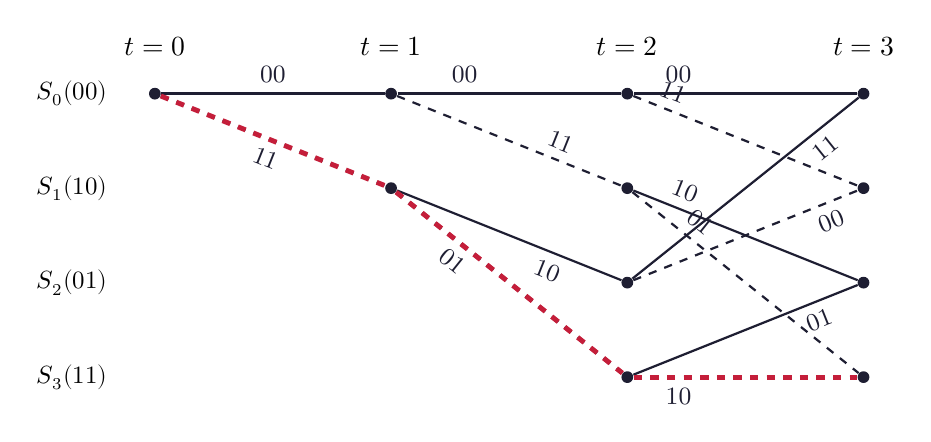
\begin{tikzpicture}[node distance=1.5cm, scale=1.2]
  % Define time steps
  \foreach \t in {0,1,2,3} {
    \node at (\t*2.5, 3.5) {\textbf{$t = \t$}};
  }
  
  % State vertical axis labels on the left
  \node[left] at (-0.4, 3) {\small $S_0(00)$};
  \node[left] at (-0.4, 2) {\small $S_1(10)$};
  \node[left] at (-0.4, 1) {\small $S_2(01)$};
  \node[left] at (-0.4, 0) {\small $S_3(11)$};

  % Draw states for each time step
  % t=0
  \node[trellisnode] (s0_0) at (0,3) {};
  
  % t=1
  \node[trellisnode] (s0_1) at (2.5,3) {};
  \node[trellisnode] (s1_1) at (2.5,2) {};
  
  % t=2
  \node[trellisnode] (s0_2) at (5,3) {};
  \node[trellisnode] (s1_2) at (5,2) {};
  \node[trellisnode] (s2_2) at (5,1) {};
  \node[trellisnode] (s3_2) at (5,0) {};
  
  % t=3
  \node[trellisnode] (s0_3) at (7.5,3) {};
  \node[trellisnode] (s1_3) at (7.5,2) {};
  \node[trellisnode] (s2_3) at (7.5,1) {};
  \node[trellisnode] (s3_3) at (7.5,0) {};

  % Draw transitions
  % t=0 to t=1
  \draw[line] (s0_0) -- node[above, sloped, pos=0.5]{\small 00} (s0_1);
  \draw[line, dashed] (s0_0) -- node[below, sloped, pos=0.5]{\small 11} (s1_1);
  
  % t=1 to t=2
  \draw[line] (s0_1) -- node[above, sloped, pos=0.3]{\small 00} (s0_2);
  \draw[line, dashed] (s0_1) -- node[above, sloped, pos=0.7]{\small 11} (s1_2);
  \draw[line] (s1_1) -- node[below, sloped, pos=0.7]{\small 10} (s2_2);
  \draw[line, dashed] (s1_1) -- node[below, sloped, pos=0.3]{\small 01} (s3_2);
  
  % t=2 to t=3
  \draw[line] (s0_2) -- node[above, sloped, pos=0.2]{\small 00} (s0_3);
  \draw[line, dashed] (s0_2) -- node[above, sloped, pos=0.15]{\small 11} (s1_3);
  
  \draw[line] (s1_2) -- node[above, sloped, pos=0.2]{\small 10} (s2_3);
  \draw[line, dashed] (s1_2) -- node[above, sloped, pos=0.25]{\small 01} (s3_3);
  
  \draw[line] (s2_2) -- node[below, sloped, pos=0.8]{\small 11} (s0_3);
  \draw[line, dashed] (s2_2) -- node[below, sloped, pos=0.85]{\small 00} (s1_3);
  
  \draw[line] (s3_2) -- node[below, sloped, pos=0.8]{\small 01} (s2_3);
  \draw[line, dashed] (s3_2) -- node[below, sloped, pos=0.2]{\small 10} (s3_3);

  % Highlight survivor path: s0_0 -> s1_1 -> s3_2 -> s3_3
  \draw[line, color=myred, line width=1.8pt, dashed] (s0_0) -- (s1_1);
  \draw[line, color=myred, line width=1.8pt, dashed] (s1_1) -- (s3_2);
  \draw[line, color=myred, line width=1.8pt, dashed] (s3_2) -- (s3_3);
\end{tikzpicture}
\end{tcolorbox}

% ===============================================================================
\section{Distance Properties of Convolutional Codes}
% ===============================================================================

The error-correcting capability of a convolutional code depends on its distance properties.

\subsection{Free Distance (\texorpdfstring{$d_{\text{free}}$}{dfree})}
The most important distance metric is the \textbf{free distance} $d_{\text{free}}$.
\begin{tcolorbox}[defbox, title={\textbf{Free Distance Definition}}]
The free distance $d_{\text{free}}$ is the minimum Hamming distance between any two distinct code sequences in the trellis that begin at state $00$ and eventually diverge, only to merge back at state $00$ at some later step.
\[ d_{\text{free}} = \min \left\{ d_H(v^{(1)}, v^{(2)}) \mid u^{(1)} \neq u^{(2)} \right\} \]
\end{tcolorbox}
If we set one sequence to be the all-zero codeword, $d_{\text{free}}$ simplifies to the minimum weight of a non-zero code sequence starting and ending at state $00$.
The number of errors $t$ that the code can correct is:
\[ t = \left\lfloor \frac{d_{\text{free}} - 1}{2} \right\rfloor \]

\subsection{Catastrophic Error Propagation}
Catastrophic error propagation is a key hazard in convolutional code design.
\begin{tcolorbox}[defbox, title={\textbf{Catastrophic Error Propagation}}]
A code is \textbf{catastrophic} if a finite number of channel transmission errors leads to an infinite number of decoding decisions/bit errors in the reconstructed message sequence.
\end{tcolorbox}
\textbf{Sufficient Condition:} In the state transition diagram of a catastrophic code, there exists a closed loop (cycle) containing a state other than $00$ where all transitions along the loop produce zero-weight output bits (all output bits are `0'), despite being triggered by non-zero inputs. 
For systematic convolutional codes, catastrophic propagation is impossible because the inputs are mirrored directly in the output stream, preventing zero-weight outputs for non-zero inputs.

% ===============================================================================
\section{The Viterbi Decoding Algorithm}
% ===============================================================================

The \textbf{Viterbi algorithm} is a Maximum Likelihood (ML) decoding technique that minimizes the probability of sequence error. It systematically searches the code trellis to find the path that is closest to the received vector.

\subsection{Algorithmic Steps}
Let the received sequence be $r = (r_0, r_1, \dots, r_{L-1})$. At each time step $t$, the decoder maintains a single survivor path for each state, along with its accumulated path metric:
\begin{enumerate}[leftmargin=*, itemsep=3.5pt]
  \item \textbf{Branch Metric (BM):} Compute the distance between the received segment $r_t$ and the expected output on each branch:
    \begin{itemize}[leftmargin=*, itemsep=2pt]
      \item \textbf{Hard Decision:} Hamming distance $d_H(r_t, v_{\text{branch}})$.
      \item \textbf{Soft Decision:} Euclidean distance $\|r_t - v_{\text{branch}}\|^2$.
    \end{itemize}
  \item \textbf{Path Metric (PM):} Calculate candidates for each state:
    \[ PM_t(S) = \min_{S' \to S} \left[ PM_{t-1}(S') + BM(S' \to S) \right] \]
  \item \textbf{Add-Compare-Select (ACS):} For each state $S$ at step $t$:
    \begin{itemize}[leftmargin=*, itemsep=2pt]
      \item \textbf{Add} branch metrics to the previous path metrics of all incoming states $S'$.
      \item \textbf{Compare} the candidate path metrics.
      \item \textbf{Select} the path with the minimum metric as the survivor. Discard all other incoming paths.
    \end{itemize}
  \item \textbf{Traceback:} Once the end of the trellis is reached (or after a fixed decoding depth), trace the path backward from the state with the lowest path metric to recover the input sequence.
\end{enumerate}

% ===============================================================================
\section{Sequential Decoding Algorithms}
% ===============================================================================

Sequential decoding algorithms are sub-optimal, tree-based decoding techniques. Unlike Viterbi, which searches all trellis paths in parallel, sequential decoders explore only one path at a time. They are suitable for codes with large constraint lengths $K$, where Viterbi's complexity ($2^{K-1}$) is prohibitive.

\subsection{Wozencraft's Algorithm}
The pioneer sequential decoding algorithm, Wozencraft's algorithm, performs a depth-first search on the code tree. It traces a path forward. If the accumulated path metric exceeds a threshold (indicating too many errors), the decoder halts, backs up (backtracks), and attempts to explore alternative branches.

\subsection{Fano's Algorithm (Fann's Algorithm)}
Fano's algorithm (referred to as Fann's in some syllabi) is a refinement of tree search that operates without a storage stack:
\begin{itemize}[leftmargin=*, itemsep=3pt]
  \item It uses a variable threshold that is dynamically adjusted based on channel quality.
  \item The decoder moves forward along the branch that maximizes the Fano metric (a metric that penalizes paths that deviate from typical channel characteristics).
  \item If the path metric falls below the threshold, the decoder lowers the threshold and backs up to explore other paths.
  \item \textbf{Advantage:} Low memory requirements. \textbf{Disadvantage:} Variable decoding time depending on channel noise.
\end{itemize}

\subsection{The Stack Algorithm (Zigangirov-Jelinek)}
The Stack (or priority queue) algorithm is a fast sequential search method:
\begin{itemize}[leftmargin=*, itemsep=3pt]
  \item The decoder maintains a list (stack) of explored paths of varying lengths, ordered by their path metrics.
  \item In each cycle, the decoder removes the path with the best metric from the top of the stack.
  \item It extends this path by computing metrics for its two child branches and inserts the new paths back into the stack.
  \item The stack is re-sorted, and the process repeats until a path reaches the end of the tree.
  \item \textbf{Advantage:} Eliminates backtracking. \textbf{Disadvantage:} Requires a large memory space to maintain and sort the stack.
\end{itemize}

% ===============================================================================
\section{Worked Example of Viterbi Decoding}
% ===============================================================================

Consider the $(2, 1, 2)$ convolutional code shown in Section 2. The encoder starts at state $S_0(00)$. We receive the sequence $r = (11, 01, 01, 00)$. Let's decode it using the Viterbi algorithm.

\subsection{Step-by-Step Trellis Computations}

\textbf{Step 1: Time $t=1$ (Received $r_0 = 11$)}\par\noindent
The only active starting state is $S_0(00)$ with path metric $PM_0(S_0) = 0$.
\begin{itemize}[leftmargin=*, itemsep=2.5pt]
  \item Transition $S_0 \to S_0$ (input 0): output $00$. $BM = d_H(11, 00) = 2$.
    $PM_1(S_0) = PM_0(S_0) + 2 = 2$. (Survivor: $S_0 \to S_0$)
  \item Transition $S_0 \to S_1$ (input 1): output $11$. $BM = d_H(11, 11) = 0$.
    $PM_1(S_1) = PM_0(S_0) + 0 = 0$. (Survivor: $S_0 \to S_1$)
\end{itemize}
States $S_2$ and $S_3$ are unreachable at $t=1$ ($PM_1 = \infty$).

\textbf{Step 2: Time $t=2$ (Received $r_1 = 01$)}\par\noindent
We transition from active states $S_0$ ($PM_1=2$) and $S_1$ ($PM_1=0$):
\begin{itemize}[leftmargin=*, itemsep=2.5pt]
  \item From $S_0$:
    \begin{itemize}[leftmargin=*, itemsep=1pt]
      \item To $S_0$ (input 0, output $00$): $BM = d_H(01, 00) = 1$. Candidate $PM = 2 + 1 = 3$.
      \item To $S_1$ (input 1, output $11$): $BM = d_H(01, 11) = 1$. Candidate $PM = 2 + 1 = 3$.
    \end{itemize}
  \item From $S_1$:
    \begin{itemize}[leftmargin=*, itemsep=1pt]
      \item To $S_2$ (input 0, output $10$): $BM = d_H(01, 10) = 2$. Candidate $PM = 0 + 2 = 2$.
      \item To $S_3$ (input 1, output $01$): $BM = d_H(01, 01) = 0$. Candidate $PM = 0 + 0 = 0$.
    \end{itemize}
\end{itemize}
Since there are no collisions yet, the survivors at $t=2$ are:
$PM_2(S_0) = 3$, $PM_2(S_1) = 3$, $PM_2(S_2) = 2$, and $PM_2(S_3) = 0$.

\textbf{Step 3: Time $t=3$ (Received $r_2 = 01$)}\par\noindent
All states are active. We apply the Add-Compare-Select (ACS) operation for each state:
\begin{itemize}[leftmargin=*, itemsep=3.5pt]
  \item \textbf{State $S_0(00)$:}
    \begin{itemize}[leftmargin=*, itemsep=1pt]
      \item From $S_0$ ($PM=3$): branch output $00$, $BM = d_H(01, 00) = 1$. Path candidate = $3 + 1 = 4$.
      \item From $S_2$ ($PM=2$): branch output $11$, $BM = d_H(01, 11) = 1$. Path candidate = $2 + 1 = 3$.
      \item \textbf{Select:} $PM_3(S_0) = \min(4, 3) = 3$. (Survivor path came from $S_2$).
    \end{itemize}
  \item \textbf{State $S_1(10)$:}
    \begin{itemize}[leftmargin=*, itemsep=1pt]
      \item From $S_0$ ($PM=3$): branch output $11$, $BM = d_H(01, 11) = 1$. Path candidate = $3 + 1 = 4$.
      \item From $S_2$ ($PM=2$): branch output $00$, $BM = d_H(01, 00) = 1$. Path candidate = $2 + 1 = 3$.
      \item \textbf{Select:} $PM_3(S_1) = \min(4, 3) = 3$. (Survivor path came from $S_2$).
    \end{itemize}
  \item \textbf{State $S_2(01)$:}
    \begin{itemize}[leftmargin=*, itemsep=1pt]
      \item From $S_1$ ($PM=3$): branch output $10$, $BM = d_H(01, 10) = 2$. Path candidate = $3 + 2 = 5$.
      \item From $S_3$ ($PM=0$): branch output $01$, $BM = d_H(01, 01) = 0$. Path candidate = $0 + 0 = 0$.
      \item \textbf{Select:} $PM_3(S_2) = \min(5, 0) = 0$. (Survivor path came from $S_3$).
    \end{itemize}
  \item \textbf{State $S_3(11)$:}
    \begin{itemize}[leftmargin=*, itemsep=1pt]
      \item From $S_1$ ($PM=3$): branch output $01$, $BM = d_H(01, 01) = 0$. Path candidate = $3 + 0 = 3$.
      \item From $S_3$ ($PM=0$): branch output $10$, $BM = d_H(01, 10) = 2$. Path candidate = $0 + 2 = 2$.
      \item \textbf{Select:} $PM_3(S_3) = \min(3, 2) = 2$. (Survivor path came from $S_3$).
    \end{itemize}
\end{itemize}

\textbf{Step 4: Time $t=4$ (Received $r_3 = 00$)}\par\noindent
We perform ACS for the final time step:
\begin{itemize}[leftmargin=*, itemsep=3.5pt]
  \item \textbf{State $S_0(00)$:}
    \begin{itemize}[leftmargin=*, itemsep=1pt]
      \item From $S_0$ ($PM_3=3$): branch output $00$, $BM = d_H(00, 00) = 0$. Path candidate = $3 + 0 = 3$.
      \item From $S_2$ ($PM_3=0$): branch output $11$, $BM = d_H(00, 11) = 2$. Path candidate = $0 + 2 = 2$.
      \item \textbf{Select:} $PM_4(S_0) = \min(3, 2) = 2$. (Survivor path came from $S_2$).
    \end{itemize}
  \item \textbf{State $S_1(10)$:}
    \begin{itemize}[leftmargin=*, itemsep=1pt]
      \item From $S_0$ ($PM_3=3$): branch output $11$, $BM = d_H(00, 11) = 2$. Path candidate = $3 + 2 = 5$.
      \item From $S_2$ ($PM_3=0$): branch output $00$, $BM = d_H(00, 00) = 0$. Path candidate = $0 + 0 = 0$.
      \item \textbf{Select:} $PM_4(S_1) = \min(5, 0) = 0$. (Survivor path came from $S_2$).
    \end{itemize}
  \item \textbf{State $S_2(01)$:}
    \begin{itemize}[leftmargin=*, itemsep=1pt]
      \item From $S_1$ ($PM_3=3$): branch output $10$, $BM = d_H(00, 10) = 1$. Path candidate = $3 + 1 = 4$.
      \item From $S_3$ ($PM_3=2$): branch output $01$, $BM = d_H(00, 01) = 1$. Path candidate = $2 + 1 = 3$.
      \item \textbf{Select:} $PM_4(S_2) = \min(4, 3) = 3$. (Survivor path came from $S_3$).
    \end{itemize}
  \item \textbf{State $S_3(11)$:}
    \begin{itemize}[leftmargin=*, itemsep=1pt]
      \item From $S_1$ ($PM_3=3$): branch output $01$, $BM = d_H(00, 01) = 1$. Path candidate = $3 + 1 = 4$.
      \item From $S_3$ ($PM_3=2$): branch output $10$, $BM = d_H(00, 10) = 1$. Path candidate = $2 + 1 = 3$.
      \item \textbf{Select:} $PM_4(S_3) = \min(4, 3) = 3$. (Survivor path came from $S_3$).
    \end{itemize}
\end{itemize}

\subsection{Traceback Process}
At the end of the trellis ($t=4$), the state with the minimum path metric is $S_1$ with $PM_4(S_1) = 0$. We trace this path backward:
\begin{enumerate}[leftmargin=*, itemsep=3pt]
  \item At $t=4$, we are in state $S_1(10)$. The survivor came from state $S_2(01)$ at $t=3$. The transition $S_2(01) \to S_1(10)$ is triggered by input bit \textbf{1}.
  \item At $t=3$, we are in state $S_2(01)$. The survivor came from state $S_3(11)$ at $t=2$. The transition $S_3(11) \to S_2(01)$ is triggered by input bit \textbf{0}.
  \item At $t=2$, we are in state $S_3(11)$. The survivor came from state $S_1(10)$ at $t=1$. The transition $S_1(10) \to S_3(11)$ is triggered by input bit \textbf{1}.
  \item At $t=1$, we are in state $S_1(10)$. The survivor came from state $S_0(00)$ at $t=0$. The transition $S_0(00) \to S_1(10)$ is triggered by input bit \textbf{1}.
\end{enumerate}
Thus, the decoded message sequence is $u = (1, 1, 0, 1)$, and the transmitted codeword is $c = (11, 01, 01, 00)$.
Since $r = c$, the accumulated Hamming distance is indeed $0$.

% ═══════════════════════════════════════════════════════════════════════════════
% QUICK REVISION PAGE
% ═══════════════════════════════════════════════════════════════════════════════
\newpage
\begin{center}
  {\large\bfseries\color{myred} Quick Revision --- Module 5}\\[3pt]
  {\small\color{mydark} Convolutional Codes and Decoding $|$ PE-EC801C}
\end{center}
\noindent{\color{myred}\rule{\linewidth}{1.2pt}}
\vspace{4pt}

\begin{tcolorbox}[formulabox, title={\textbf{Key Formulas and Metrics at a Glance}}]
\renewcommand{\arraystretch}{1.35}
\begin{tabularx}{\linewidth}{B{5.0cm} X}
Code Rate & $R = \displaystyle\frac{k}{n}$ \\[4pt]
Constraint Length (Standard) & $K = M + 1$ \quad ($M$ is the number of delay stages) \\[4pt]
Impulse Response Convolution & $v^{(j)}_t = \sum_{i=0}^M u_{t-i} h^{(j)}_i$ \\[4pt]
Discrete Delay Polynomial & $g^{(j)}(D) = g^{(j)}_0 \oplus g^{(j)}_1 D \oplus \dots \oplus g^{(j)}_M D^M$ \\[4pt]
Error Correction Power & $t = \left\lfloor \displaystyle\frac{d_{\text{free}} - 1}{2} \right\rfloor$ \\[4pt]
Viterbi Path Metric Update & $PM_t(S) = \min_{S' \to S} \left[ PM_{t-1}(S') + BM(S' \to S) \right]$
\end{tabularx}
\end{tcolorbox}

\vspace{6pt}

\begin{tcolorbox}[defbox, title={\textbf{One-Line Definitions}}]
\begin{itemize}[leftmargin=*, itemsep=3.5pt, topsep=0pt]
  \item \textbf{Convolutional Code:} A continuous coding technique where outputs are generated by convolving current and past message bits.
  \item \textbf{Constraint Length ($K$):} The number of input bits that reside in the encoder and influence the output.
  \item \textbf{Trellis Diagram:} A time-indexed state diagram showing all possible transitions over time.
  \item \textbf{Free Distance ($d_{\text{free}}$):} The minimum Hamming distance between any two distinct paths in the trellis starting and ending in $00$.
  \item \textbf{Catastrophic Code:} A code where a finite number of channel errors causes an infinite number of decoded bit errors.
  \item \textbf{Survivor Path:} The path entering a trellis state that has the minimum accumulated path metric.
  \item \textbf{ACS (Add-Compare-Select):} The core hardware operation in Viterbi decoding that updates path metrics and retains survivors.
  \item \textbf{Fano Metric:} A dynamic search metric that penalizes paths that deviate from typical channel behavior.
\end{itemize}
\end{tcolorbox}

\newpage

\begin{tcolorbox}[exambox, title={\textbf{Frequently Asked / Viva Questions}}]
\begin{enumerate}[topsep=0pt, label=\textbf{Q\arabic*.}, itemsep=5pt]
  \item \Q{What is the difference between block codes and convolutional codes?}
    Linear block codes process messages in independent block segments, and the current output block depends only on the current input block. Convolutional codes process the input continuously, and the output depends on the current input and a finite memory of past inputs.
  \item \Q{Define constraint length $K$ in a convolutional encoder.}
    Constraint length $K$ represents the number of input cycles over which an input bit remains in the shift register and influences the output. It is mathematically defined as $K = M + 1$, where $M$ is the number of memory delay elements.
  \item \Q{What is free distance $d_{\text{free}}$ and why is it important?}
    Free distance $d_{\text{free}}$ is the minimum Hamming distance between any two paths in the trellis that diverge from the all-zero state and merge back later. It determines the code's error-correcting capability: $t = \lfloor(d_{\text{free}}-1)/2\rfloor$.
  \item \Q{How do you identify a catastrophic convolutional code from its state diagram?}
    A code is catastrophic if its state transition diagram contains a loop of non-zero states where all outputs are zero. If transmission errors cause the decoder to enter this loop, it will continue to output errors indefinitely.
  \item \Q{State the three structural representations of convolutional codes.}
    The three structural representations are the State Transition Diagram (FSM representation), the Tree Diagram (exponential tree branching showing all output sequences), and the Trellis Diagram (compact time-aligned state transitions).
  \item \Q{Explain the ACS operation in the Viterbi algorithm.}
    ACS stands for Add-Compare-Select. For each trellis state, it adds the branch metrics of incoming branches to the path metrics of their origin states, compares the candidate values, and selects the path with the minimum metric as the survivor.
  \item \Q{What is the difference between hard-decision and soft-decision decoding?}
    Hard-decision decoding processes demodulated binary data (`0' or `1') and uses Hamming distance. Soft-decision decoding processes unquantized analog voltage values directly from the channel and uses Euclidean distance, offering a 2--3 dB coding gain.
  \item \Q{Compare Viterbi decoding with sequential decoding.}
    Viterbi decoding is a maximum likelihood algorithm that searches all trellis paths in parallel, requiring $2^M$ state processors. Sequential decoding explores a single path at a time in a tree structure, using backtracking or stacks, which reduces memory but introduces variable decoding delays.
  \item \Q{How does Fano's sequential decoding algorithm work?}
    Fano's algorithm performs a tree search by moving forward or backward along branches based on a metric threshold. If the path metric falls below the threshold, it lowers the threshold and backtracks, requiring no memory stacks.
  \item \Q{What is the Stack algorithm, and what is its main drawback?}
    The Stack algorithm (Zigangirov-Jelinek) maintains a priority queue of paths ordered by their metrics, extending the top path. Its main drawback is the large memory required to store and sort the paths, and the risk of stack overflow under noisy conditions.
\end{enumerate}
\end{tcolorbox}

\vspace{6pt}

\begin{tcolorbox}[tikzbox, title={\textbf{Structural Comparison of Block and Convolutional Codes}}]
\renewcommand{\arraystretch}{1.45}
\begin{tabularx}{\linewidth}{|B{3.2cm}|Y|Y|}
\hline
\textbf{Property} & \textbf{Linear Block Codes} & \textbf{Convolutional Codes} \\
\hline
Encoding Mode & Block-by-block (independent segments) & Continuous stream processing \\
\hline
Memory Structure & Memoryless (outputs depend on current block) & Finite memory (outputs convolved with history) \\
\hline
Key Parameters & Code length $n$, message length $k$ & Rate $k/n$, constraint length $K$, memory $M$ \\
\hline
Decoding Algorithm & Syndrome table lookup / Meggitt decoding & Viterbi / Sequential decoding \\
\hline
\end{tabularx}
\end{tcolorbox}

\vspace{6pt}

\begin{tcolorbox}[tikzbox, title={\textbf{Comparison of Viterbi vs. Sequential Decoding}}]
\renewcommand{\arraystretch}{1.45}
\begin{tabularx}{\linewidth}{|B{3.2cm}|Y|Y|}
\hline
\textbf{Property} & \textbf{Viterbi Decoding} & \textbf{Sequential Decoding} \\
\hline
Search Strategy & Parallel search over all trellis paths & Single-path depth-first tree search \\
\hline
Optimality & Maximum Likelihood (optimal) & Sub-optimal \\
\hline
Decoding Time & Constant (independent of channel noise) & Variable (increases with channel noise) \\
\hline
Constraint Limit & Limited to small $K$ ($K \le 9$) & Can decode large $K$ ($K \ge 20$) \\
\hline
Memory Demand & Low storage (only survivor paths) & High storage (stack) or backtracking overhead \\
\hline
\end{tabularx}
\end{tcolorbox}

\end{document}
